\chapter{INTRODUCTION}

Relief sculpting has been practiced for thousands of years.Since antiquity, artisans from many ancient cultures(including Greek, Persian, Egyptian, Mayan, and Indian art) have created bas-reliefs (Figure \ref{bas:his}).Today bas-reliefs are commonly found in a variety of media in architecture, industrial design and coins. However, the production of bas-reliefs is currently a costly and time-consuming process, requiring skilled sculptors and engravers.Even with the advent of computer-driven techniques providing a foundation for automation in bas-relief, making the design of bas-relief sculptures remains largely in the hands of artists.

As an artistic form, relief spans the continuum between a 2D  painting and a full 3D sculpture\cite{weyrich2007digital}. On this spectrum, alto-relievo (high relief) is closest to full 3D, whereas flatter artworks are described as basso-relievo (low relief, and also called bas-relief), as showed in Figure \ref{bas:his}. Among all the sculpture forms, bas-relief is arguably the closest to 2D paintings, as claimed by\cite{kerber2009feature} and\cite{barron2012color}.
 
\begin{figure}[H]
	\centering
	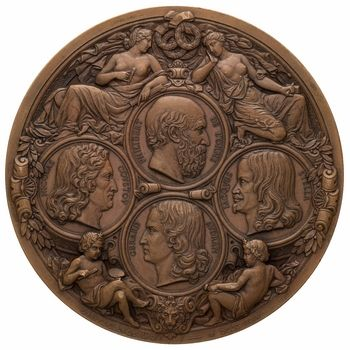
\includegraphics[height=0.2\textheight]{bas.jpg}
	~~~~
	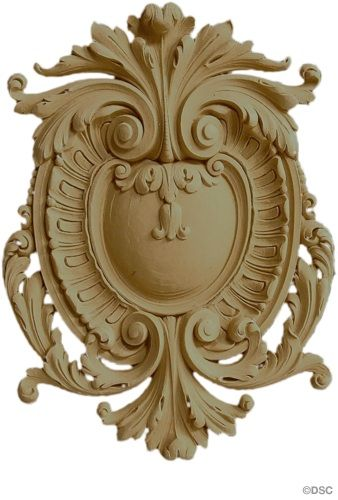
\includegraphics[height=0.2\textheight]{bas2.jpg}
	\caption{Bas-relief}
	\label{bas:his}  
\end{figure} 

Currently, most existing bas-relief production methods focus on compressing 3D scenes/models into surfaces with a small depth\cite{weyrich2007digital}and\cite{kerber2009feature}. This approach requires a 3D model as a starting point. 

Another option is to generate bas-reliefs directly from 2D images.There have been some image based bas-relief production approaches avail	able in\cite{zeng2014region}\cite{wu2013making} and \cite{alexa2010reliefs}. These approaches almost follow the “bas-relief ambiguity”\cite{belhumeur1999bas}, that is, roughly speaking, from a frontal view the sculpture looks like a full 3D object while a side-view reveals the disproportional depth. 

While most image based method are focusing on general photograph, which unsuited for specific problems for brush paintings, such as spatial occlusion (i.e. one stroke occludes other strokes in the paining to demonstrate the depth perception) and stroke transparency. A another clear shortcoming is current image based methods can’t take the artistic intent into account, as all what they do is to inferring the height information from the image. Concerning reproduction or modifying of an artistic painting, it is crucial that the style of the originals is preserved, which is not considered in existing image-based methods. However, little is done in the area of bas-relief generation from artistic paintings, as maintaining the styles of the brush paintings proves much trickier than simply manipulating the height of the contour lines. In the case of bas-reliefs, although there is no 3D model available, pseudo 3D effect reflecting the style and subtlety is crucial in preserving the artistic essence.

The aim of our research is to provide the bas-relief sculptors with a new tool allowing them to convert and recompose existing brush paintings to bas-reliefs. We also argue that because traditional paintings are produced with individual strokes, ‘3D bas-relief strokes’ will enable them to ‘paint/sculpt’ a bas-relief naturally, especially if they wanted to quickly convert an existing painting into a relief. With the commonly and cheaply available 3D printing facilities, there is a growing trend in the need of bas-relief art products.
A brush painting can be regarded as the union of a set of hypothetical strokes by a brush \cite{xu2006animating}. Differing from the other bas-relief generation methods, our method will honor this very feature by constructing the brush strokes individually as 3D geometric entities. This however demands to conquer several challenges. First, each brush stroke covers a region on the canvas and they may overlap each other, some quite heavily in a painting. To make sure the information is retained, every stroke has to be faithfully extracted. Second, spatial occlusion has to be dealt with, since artists are used to depicting it through controlling the transparency of strokes as one of the art elements. Third, as an artistic tool, the generated bas-relief should be further editable allowing the artist to rearrange, tweaking and reshaping the extracted strokes.

The shape, color and opacity of a stroke vary due to the shape and firmness of the brush as well as the forces the artist imposes. Although these variables add the complexity to stroke extraction, stylized strokes often follow distinct patterns. For example, Rosemaling paintings, a typical example of brush painting popular in North Europe, is a traditional form of decorative folk art that originated in the rural valleys of Norway. The Rosemailing designs use C and S strokes, feature scroll, flowing lines, floral designs, and both subtle and vibrant colors. The brush strokes may further be viewed as graphical objects which are meaningful with respect to the objects the painting portraits. Moreover, each stroke is clearly visible due to both subtle and vibrant colors. The similar properties may be found in some Chinese brush paints.
To extract the strokes from a brush painting, we need to identify and segment the overlapped strokes. We will then generate the depth map for every stroke separately using the shape from shading (SFS) technique on the opacity. All the strokes are finally merged together to yield the resulting bas-relief with the original 2D painting preserved. Our contributions include,
\newline
(1) Extraction of brush strokes. We develop a novel method to extract brush strokes from input paintings with palette analysis and decomposed layers.
\newline
(2) 3D modeling of brush strokes. We develop a novel method which may entirely construct every stroke in 3D based on the opacity of paintings.
\newline
(3) Recomposition in bas-relief design. Artists may redefine the brush strokes’ order and shapes by sketches, which enable recomposition in bas-relief design, making it a useful tool for sculpture artists.



\section{Thesis Structure}

The organization of the document is as follows:

Chapter 1: Introduction. This section provides the background, the motivation and the contribution made in current research.

Chapter 2: Literature Review. This section classifies and reviews related previous works  in a systematic way.

Chapter 3: Overview of proposed approach. This section explains the methodology selected and defines some basic concepts used in the research.

Chapter 4: Layer Decomposition. This section introduces concept "Layer Decomposition" in this research, which is the basis of the proposed algorithm.

Chapter 5: Extraction of Brush strokes. This section describes the proposed algorithm of brush stroke extraction.

Chapter 6: Depth map and '3D strokes'.  This section shows how to generate the individual depth maps of extracted strokes. 

Chapter 7: Results. This section reviews the up-to-date results based on proposed the method.

Chapter 8: Conclusions . This section concludes the progress up-to-date.

Chapter 9: Future work. This section discusses possible future work about high relief and 3D painting.
